\chapter{Método de Trabajo}
\label{chap:metodo}

\drop{D}{urante} toda la extensión de este capítulo, se ahondará en las metodologías que se han utilizado para la realización de este \acs{TFM}. En este caso, el marco de trabajo para la gestión de proyectos escogido ha sido Scrum, mientras que la metodología de desarrollo de software ha sido la del ciclo de vida iterativo e incremental. Scrum, al poseer artefactos como el \textit{Product Backlog} o eventos como el Sprint, junto con las reuniones diarias y las revisiones de los Sprints, se convierte en una de las mejores candidatas a aplicar a este trabajo. Por tanto, se ha realizado una interpretación de dicha metodología con el fin de poder adaptarla y adoptarla durante el desarrollo del \acs{TFM}.

\section{Scrum, una metodología de gestión de proyectos}
Scrum no se trata de una abreviatura de un término, sino de un concepto para la gestión de proyectos. Describe cómo un equipo puede implementar con mayor rapidez procesos complejos de desarrollo cuando este se encuentra formado por pequeñas unidades auto-organizadas \cite{robertmulsow2018}. Se encuentra enfocado al uso de un proceso empírico que permite a los equipos responder con rapidez, eficiencia y eficacia al cambio \cite{michelesliger}. Dentro de este, es posible utilizar diferentes procesos y técnicas, dividiendo el proyecto en diferentes fases, de manera que una no puede comenzar si la anterior no ha finalizado \cite{scrumguide}.

\subsection{Pilares de Scrum}
Como se ha comentado anteriormente, se enfoca al uso de un proceso empírico (teoría de control de procesos empírica), obteniendo el conocimiento a partir de la experiencia adquirida de la toma de decisiones pasadas. Además, posee tres conceptos en torno a los que se desarrolla \cite{scrumguide}:

\begin{itemize}
    \item \textbf{Transparencia}. Esto representa que los aspectos importantes del proceso han de ser visibles a las personas que son responsables del resultado.
    \item \textbf{Inspección}. Este segundo concepto tiene que ver con la detección de desviaciones. Es decir, enfocándose en una meta concreta, los usuarios de Scrum han de revisar los artefactos que se vayan produciendo con el fin de detectar posibles variaciones no deseadas.
    \item \textbf{Adaptación}. No obstante, en el caso de que se haya producido alguna desviación indeseada, si un inspector determina que se han superado los límites aceptables, el proceso ha de ser reajustado en el plazo más breve posible para evitar una desviación mayor.
\end{itemize}

\subsection{El marco de trabajo de Scrum}
Scrum provee una estructura para la entrega de resultados, no las prácticas específicas que se deben seguir, aspecto que se deja a libre elección. Por tanto, define un marco de trabajo que se muestra en la Figura \ref{fig:scrum_framework} \cite{scrumframewok}. A continuación, se procederá a detallar este marco, indicando los diferentes roles y responsabilidades que se pueden encontrar dentro de Scrum, así como los eventos y artefactos de los que se compone.

\begin{figure}[h]
  \centering
  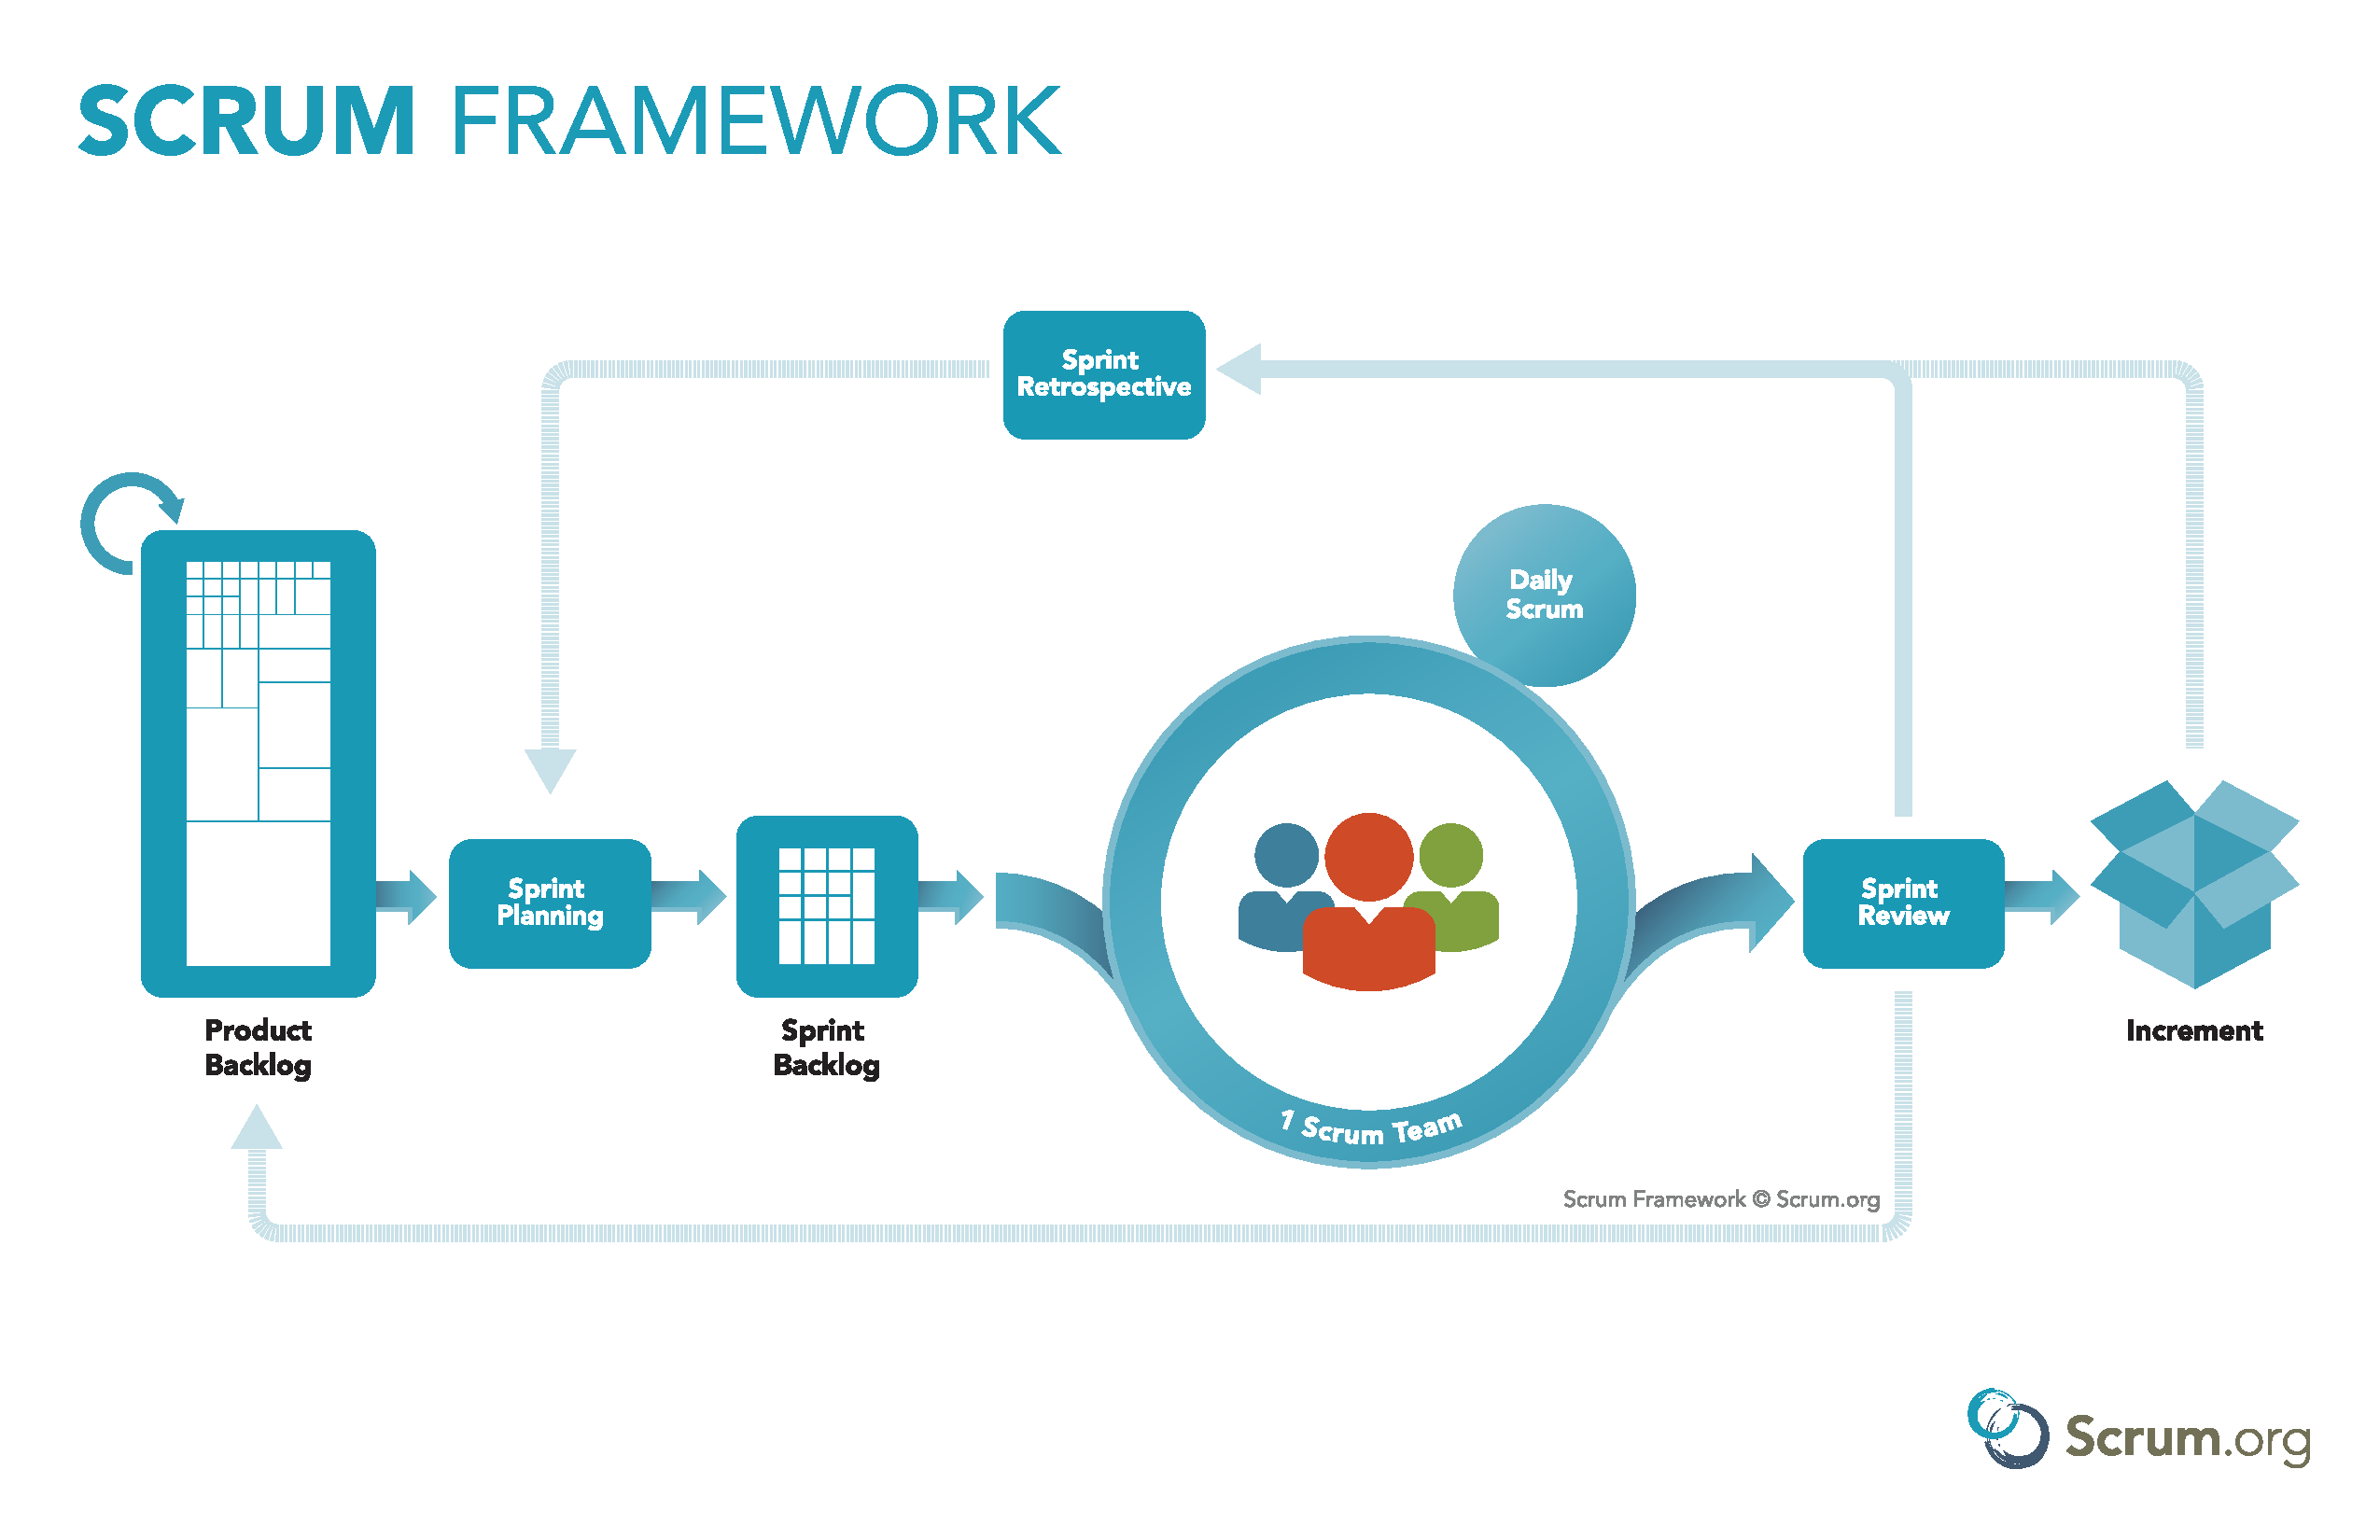
\includegraphics[width=0.8\linewidth]{figures/images/ScrumFramework.pdf}
  \caption{Marco de trabajo de Scrum}
  \source{\url{https://www.scrum.org/index.php/resources/scrum-framework-poster}}
  \label{fig:scrum_framework}
\end{figure}

\clearpage

\subsection{Roles y responsabilidades}
En Scrum existen tres roles principales: el Maestro de Scrum (\textit{Scrum Master}), el Dueño del Producto (\textit{Product Owner}) y el Equipo de Scrum (\textit{Scrum Team}).

\subsubsection{Maestro de Scrum (\textit{Scrum Master})}
Esta persona será la responsable de asegurar que todos los procesos se siguen correctamente, además de ejercer como defensor y protector del equipo ante amenazas o interferencias externas. Asegura y facilita la comunicación en el equipo, elimina obstáculos o media en las posibles discusiones que puedan aparecer. En definitiva, se trata de un <<facilitador>>.

\subsubsection{Dueño del Producto (\textit{Product Owner})}
Esta figura actúa en representación de los interesados (\textit{stakeholders}) del proyecto, siendo la voz de estos y con la capacidad de tomar decisiones sobre el producto. Realiza las funciones de mediador entre el equipo y el dueño del producto. Por otra parte, tiene el control sobre la Pila del Proyecto (\textit{Product Backlog}), por lo que también es el responsable de la definición, priorización o la correcta descripción de los elementos de los que esté compuesta.

\subsubsection{Equipo de Scrum (\textit{Scrum Team})}
Como regla general, el Equipo de Scrum ha de estar compuesto por siete más menos dos personas, que serán las encargadas de la entrega del producto y trabajarán sobre las diferentes tareas a realizar. Mientras que el Dueño del Producto se encarga del <<qué>>, el Equipo de Scrum se encarga del <<cómo>>. Su función última es la de entregar un incremento del producto terminado al final de cada Sprint. Las características más relevantes del Equipo de Scrum son las siguientes \cite{scrumguide}:

\begin{itemize}
    \item \textbf{Son autoorganizados}. La estructura y el modo de trabajo se conforman sin intervención externa explícita.
    \item \textbf{Son multifuncionales}. El conjunto de todos los miembros cuenta con las habilidades necesarias para desarrollar un incremento.
    \item \textbf{No se reconocen títulos individuales}. La responsabilidad de trabajo se asume por parte del equipo como unidad, es decir, el grupo es más importante que el individuo.
    \item \textbf{No se reconocen subequipos}. Este punto podría considerarse como una derivación del anterior, donde se indica que el grupo cuenta con mayor relevancia.
    \item \textbf{Cada miembro ha de tener habilidades especializadas y áreas en las que enfocarse}. Aunque es importante que cada miembro cuente con habilidades específicas, la responsabilidad final siempre recaerá sobre el conjunto del equipo.
\end{itemize}

\subsection{Eventos de Scrum}
Scrum se compone también de una serie de eventos que  se organizan en torno a bloques de tiempo o Sprints con el fin de crear un hábito y continuidad en el trabajo.

\subsubsection{El Sprint}
Este es el elemento principal en torno al que gira Scrum. Se trata de un bloque de tiempo con una duración fija y no superior a un mes dentro del que se desarrolla un entregable o incremento. Además, los Sprints no podrán solaparse puesto que son consecutivos, es decir, no puede dar comienzo uno nuevo mientras el actual aún no ha terminado.


\subsubsection{Planificación del Sprint (\textit{Sprint Planning Meeting})}
Se trata de una reunión que se lleva a cabo en el primer día de cada Sprint con la finalidad de programar el trabajo a realizar durante el mismo y a la que atienden todos los roles de Scrum. En ella, el Dueño del Producto presenta todo lo que le gustaría ver completado y, entonces, el Equipo de Scrum determina las tareas a realizar. La reunión ha de finalizar con un \textit{Sprint Backlog}, un propósito para el Sprint, el compromiso del equipo y su estimación del esfuerzo requerido, además de la correcta comprensión de todas las tareas a realizar por parte de cada integrante.

\subsubsection{Scrum Diario (\textit{Daily Scrum})}
Este evento consta de una reunión de corta duración en la que se revisan las tareas realizadas, las que hay que realizar y se sincronizan las actividades. Además, se expone tanto lo que se ha realizado el día anterior como lo que se va a realizar en esa jornada y los impedimentos o problemas que pudieran haberse presentado. Con la intención de dotar al proyecto de una mayor agilidad, se ha optado por hacer uso de Microsoft Teams, donde se dispone de un canal con el mismo nombre dedicado a exponer todas esas cuestiones, obteniendo un \textit{feedback} cuando sea necesario.

\subsubsection{Revisión del Sprint (\textit{Sprint Review}) y Retrospectiva del Sprint (\textit{Sprint Retrospective})}
La Revisión del Sprint es una reunión que se realiza al final de cada Sprint en la que el equipo convoca a los interesados para obtener \textit{feedback} a partir del entregable realizado. También, si fuera necesario, se ajustaría la Pila de Producto. Una vez que la revisión ha finalizado, el equipo lleva a cabo una retrospectiva con la finalidad de valorar el trabajo realizado durante el Sprint, de manera que se pueda crear un plan de mejora antes de la siguiente planificación.


\clearpage


\subsection{Artefactos de Scrum}
En Scrum, los llamados <<artefactos>> representan valor o trabajo y proporcionan transparencia a todas las personas implicadas en el proyecto. Estos artefactos se exponen a continuación \cite{scrumguide}.

\subsubsection{Pila del Producto (\textit{Product Backlog})}
Se trata de una lista ordenada en la que se incluye todo lo que va a ser necesario, y cuyo responsable es el Dueño del Producto. Es dinámica y suele estar sujeta a cambios, incluyendo las características, funciones, requisitos, mejoras y correcciones.

\subsubsection{Pila del Sprint (\textit{Sprint Backlog})}
Derivación del anterior artefacto, la Pila del Sprint se conforma a partir de la Pila del Producto y contiene todos los trabajos que se han de realizar en un determinado Sprint. De igual manera, es dinámica y se va modificando conforme avanza el Sprint.

\subsubsection{Incremento}
El incremento es la suma de todos los elementos que se han completado en el Sprint y el valor que aportan los Sprints anteriores.

\clearpage

\subsection{Aplicación de SCRUM al proyecto}
Finalmente, se detallarán las adaptaciones que se han realizado para poder adoptar la metodología durante la totalidad del desarrollo del presente \acs{TFM}.

\subsubsection{Aplicación de los diferentes roles y responsabilidades}
Debido a la naturaleza del trabajo y del reducido tamaño del equipo de Scrum, se han establecido los diferentes actores dentro del proyecto, quedando los roles identificados de la siguiente manera:

\begin{itemize}
    \item \textbf{Dueño del Producto}: Andrés Javier Prado Domínguez.
    \item \textbf{Maestro de Scrum}: Luis Rodríguez Benítez.
    \item \textbf{Equipo de Scrum}: Diego Andérica Richard.
\end{itemize}

\subsubsection{Aplicación de los eventos al \acs{TFM}}
Teniendo todo lo anterior en cuenta, para este trabajo se ha definido una duración de Sprint de dos semanas. No obstante, se desarrollará un primer Sprint denominado <<Sprint 0>> donde se fijarán los pilares del trabajo por lo que, teniendo en cuenta su naturaleza y el carácter del proyecto, como se expondrá más adelante, se definió la duración de este en una semana.

En cuanto al resto de eventos de Scrum, con el fin de poder adoptarlos en este proyecto, se han fijado reuniones todos los viernes con una duración estimada de unos 45 minutos a las que se ha denominado como <<reuniones de seguimiento>>. Puesto que el Sprint tiene una duración de dos semanas, cada uno contendrá un total de dos reuniones, donde en una de ellas se realizará un seguimiento, mientras que la otra servirá para realizar la Revisión del Sprint que acaba de finalizar, así como la planificación del próximo.

\subsubsection{Aplicación de los artefactos al \acs{TFM}}
En cuanto a la adopción de los artefactos de Scrum, tanto para la Pila del Producto como para la Pila del Sprint se hará uso de Microsoft Planner, moviendo las tareas de la Pila de Producto al correspondiente bloque del Sprint.


\clearpage


\section{Ciclo de vida iterativo e incremental}
El ciclo de vida del software abarca desde la concepción de la idea de este hasta la finalización de su uso, incluyendo los diferentes estados por los que pasa en etapas intermedias. Este ciclo de vida se encuentra ligado a Scrum por tratarse de una metodología ágil y consiste en el desarrollo por partes del producto, integrando estas partes de manera progresiva conforme se van completando. Constituye una de las bases de un proyecto ágil puesto que se cuenta con iteraciones cortas en el tiempo \cite{javiergarzas2012}, de manera que el producto final va adquiriendo una mayor funcionalidad y, por tanto, una mayor calidad final. Por otra parte, en cada iteración se revisa y mejora el producto, añadiendo nuevos requisitos o mejorando los ya existentes \cite{proyectosagiles}. En cierto modo, se crean proyectos más pequeños entre los que se reparte el trabajo total donde cada uno representa una iteración que generará un incremento como resultado. Todos estos proyectos derivados siguen el esquema análisis-diseño-pruebas (Figura \ref{fig:iteraincr}), lo que deriva en una serie de ventajas: el riesgo del proyecto se ve acotado a un incremento, permite concentrar el esfuerzo de los desarrolladores para mejorar la eficiencia en cada iteración y se puede conseguir una mejor especificación de los requisitos.

\begin{figure}[h]
  \centering
  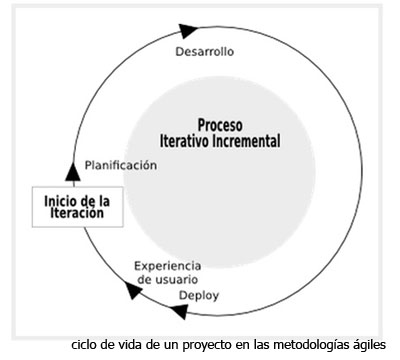
\includegraphics[width=0.52\linewidth]{figures/images/ciclo_iterativo_incremental.jpg}
  \caption{Ciclo Iterativo e Incremental}
  \source{\url{https://commons.wikimedia.org/wiki/File:Ciclo_de_vida_proyecto_metodologia_agiles.jpg}}
  \label{fig:iteraincr}
\end{figure}

\clearpage

\section{Planificación de los Sprints}
A continuación, se comenzará presentando la planificación, los trabajos desarrollados y las reuniones que han tenido lugar en cada Sprint para, posteriormente, exponer los resultados obtenidos de manera global. En primer lugar, se detallará el Sprint 0, exponiendo el porqué de su uso en este trabajo.

\subsection{Sprint 0: planificación inicial y adaptación de Scrum}
El primer Sprint que se ha desarrollado es el Sprint 0. Durante el desarrollo de este Sprint no se produce ningún incremento ni entregable, por lo que no se ajustaría a la definición de Sprint como tal. A pesar de esto, se considera que tampoco es erróneo su desarrollo e inclusión en la metodología del proyecto \cite{alexballarinlatre2017}. Por tanto, no posee carácter obligatorio aunque resulta de utilidad ya que se encuentra orientado a la preparación y a sentar las bases del proyecto que se va a realizar. Estas bases pueden ser algunos artefactos como el \textit{Product Backlog}, la duración de los diferentes eventos o la definición de los objetivos \cite{agripinopetit2017}. Por tanto, la primera reunión tuvo lugar el día 28-06-19 con el objetivo de establecer la metodología y sentar las bases del proyecto.

\subsubsection{Pila de Producto}
La Tabla \ref{tab:pilaproducto} representa la Pila de Producto del proyecto, que contiene todas las tareas que se deben realizar durante el desarrollo del mismo, de manera que los objetivos fijados se vean satisfechos. Esta tabla se ha ido definiendo a lo largo de las reuniones mantenidas con todos los involucrados en el proyecto, estableciendo un total de 25 ítems.

\begin{table}[!htbp]
	\centering
	{\small
		\begin{tabular}{|l|l|l|}
	\hline
	\multicolumn{3}{|c|}{\cellcolor[HTML]{343434}{\color[HTML]{FFFFFF} \textbf{Pila de Producto}}} \\ \hline
	\textbf{ID} & \textbf{Nombre} & \specialcell{\textbf{Duración} \\ \textbf{Estimada (h)}} \\ \hline
	1  & Redacción del Resumen                                      & 5  \\ \hline
	2  & Redacción capítulo de Introducción                         & 5  \\ \hline
	3  & Redacción capítulo de Objetivos                            & 10 \\ \hline
	4  & Redacción capítulo de Antecedentes                         & 25 \\ \hline
	5  & Redacción capítulo de Metodología                          & 10 \\ \hline
	6  & Realizar análisis del entorno general                      & 30 \\ \hline
	7  & Realizar análisis del entorno específico                   & 30 \\ \hline
	8  & Estudio de ventajas competitivas de un servicio \acs{DaaS} & 20 \\ \hline
	9  & Definición de un modelo de negocio basado en \acs{DaaS}    & 20 \\ \hline
	10 & Creación del servicio de \acs{WVD}                         & 10 \\ \hline
	11 & Creación de un \textit{hostpool} en \acs{WVD}              & 10 \\ \hline
	12 & Desarrollo de una aplicación para la gestión de \acs{WVD}  & 35 \\ \hline
	13 & Documentación de la aplicación de gestión                  & 15 \\ \hline
	14 & Realización de casos de uso                                & 30 \\ \hline
	15 & Documentación de los casos de uso                          & 15 \\ \hline
	16 & Realización de un análisis comparativo                     & 20 \\ \hline
	17 & Redacción capítulo de Conclusiones y Trabajos Futuros      & 10 \\ \hline
	18 & Revisión completa del documento                            & 20 \\ \hline
	19 & Documentación Sprint 1                                     & 5  \\ \hline
	20 & Documentación Sprint 2                                     & 5  \\ \hline
	21 & Documentación Sprint 3                                     & 5  \\ \hline
	22 & Documentación Sprint 4                                     & 5  \\ \hline
	23 & Documentación Sprint 5                                     & 5  \\ \hline
	24 & Documentación Sprint 6                                     & 5  \\ \hline
	25 & Documentación Sprint 7                                     & 5  \\ \hline
\end{tabular}
	}
	\caption[Pila de Producto]
	{Pila de Producto}
	\label{tab:pilaproducto}
\end{table}

\clearpage

\subsection{Sprint 1}
El Sprint 1 se ha desarrollado desde el día 08-07-19 hasta el 21-07-19 y durante estas dos semanas se han realizado diferentes tareas que se pueden clasificar como <<documentación>>, <<desarrollo>> e <<investigación>>. En la reunión que tuvo lugar el día 03-07-19 se establecieron las tareas a realizar dentro del desarrollo de este Sprint, así como la definición de los objetivos y la aprobación de las adaptaciones de la metodología a utilizar. A partir de la Pila de Producto, conformada en el Sprint 0, se extrajeron las tareas a realizar para crear la Pila del Sprint, que se muestra en la Tabla \ref{tab:pilasprint1}.

\begin{table}[!htbp]
	\centering
	{\small
		\begin{tabular}{|l|l|l|l|}
	\hline
	\multicolumn{4}{|c|}{\cellcolor[HTML]{343434}{\color[HTML]{FFFFFF} \textbf{Pila de Sprint 1}}} \\ \hline
	\textbf{ID} & \textbf{Nombre} & \specialcell{\textbf{Duración} \\ \textbf{Estimada (h)}} & \textbf{Prioridad} \\ \hline
	2  & Redacción capítulo de Introducción    & 5  & Normal     \\ \hline
	3  & Redacción capítulo de Objetivos       & 10 & Crítico    \\ \hline
	4  & Redacción capítulo de Antecedentes    & 25 & Normal     \\ \hline
	5  & Redacción capítulo de Metodología     & 10 & Crítico    \\ \hline
	10 & Creación del servicio de \acs{WVD}    & 10 & Importante \\ \hline
	6  & Realizar análisis del entorno general & 30 & Crítico    \\ \hline
	19 & Documentación Sprint 1                & 5 & Normal      \\ \hline
\end{tabular}
	}
	\caption[Pila de Sprint 1]
	{Pila de Sprint 1}
	\label{tab:pilasprint1}
\end{table}

\subsubsection{Reunión de seguimiento}
El día 12-07-19 se llevó a cabo una reunión de seguimiento donde se expusieron los avances realizados durante la primera semana del Sprint. En ella, además, se han definido las tareas que debían comenzar durante la segunda semana y se decidió devolver la redacción del capítulo de Antecedentes, posponiéndola a etapas más avanzadas del proyecto.

\subsubsection{Revisión del Sprint}
Debido a un imprevisto, la reunión correspondiente a este evento de la metodología tuvo que ser pospuesta a la mañana del día 22-07-19. En esta reunión se ha revisado la redacción de los diferentes capítulos expuestos en la Pila del Sprint, a excepción del capítulo de Antecedentes que, como se acordó en la reunión de seguimiento, se pospondrá para futuros sprints. Fruto de esta revisión, se deberán realizar algunas correcciones en la redacción del documento, así como devolver a la Pila de Producto la realización del análisis general. Una vez que dé comienzo el Sprint 2, se extraerá de nuevo esta tarea para ser finalizada.

\clearpage

\subsection{Sprint 2}
El Sprint 2 se ha llevado a cabo desde el día 22-07-19 al 02-08-19 y se han realizado tareas tanto de documentación como de investigación y técnicas. El día 22-07-19 se realizó la reunión de planificación del Sprint, donde se ha determinado el conjunto de tareas que se deben acometer durante las próximas dos semanas (Pila del Sprint), que se ven reflejadas en la Tabla \ref{tab:pilasprint2}. Como se observa en dicha tabla, la tarea <<realizar análisis del entorno general>> ya se encontraba en la Pila del Sprint 1 pero, puesto que no se ha conseguido terminar, se ha decidido devolver a la Pila del Producto para rescatarla y finalizarla en la Pila del Sprint 2, de ahí que la estimación de la duración sea inferior.

\begin{table}[!htbp]
	\centering
	{\small
		\begin{tabular}{|l|l|l|l|}
	\hline
	\multicolumn{4}{|c|}{\cellcolor[HTML]{343434}{\color[HTML]{FFFFFF} \textbf{Pila de Sprint 2}}} \\ \hline
	\textbf{ID} & \textbf{Nombre} & \specialcell{\textbf{Duración} \\ \textbf{Estimada (h)}} & \textbf{Prioridad} \\ \hline
	6  & Realizar análisis del entorno general          & 10 & Crítico    \\ \hline
	7  & Realizar análisis del entorno específico       & 30 & Crítico    \\ \hline
	11 & Creación de un \textit{hostpool} en \acs{WVD}  & 10 & Importante \\ \hline
	1  & Redacción del Resumen                          & 5  & Normal     \\ \hline
	20 & Documentación Sprint 2                         & 5  & Normal     \\ \hline
\end{tabular}
	}
	\caption[Pila de Sprint 2]
	{Pila de Sprint 2}
	\label{tab:pilasprint2}
\end{table}

\subsubsection{Reunión de seguimiento}
Debido a imprevistos externos, la reunión de seguimiento planificada para el viernes, día 26 de julio de 2019, no pudo ser llevada a cabo. Ante esta situación, se decidió posponer al martes, día 30 de julio de 2019. El objetivo de esta reunión era poner en conocimiento de los involucrados los avances realizados, así como fijar las tareas a realizar durante los próximos Sprints, puesto que estos se desarrollarán durante el periodo estival.

\subsubsection{Revisión del Sprint}
La reunión de revisión, planificada para el día 2 de agosto de 2019 no se ha podido desarrollar como estaba previsto, pues esta se encuentra ya dentro del periodo vacacional. En consecuencia, la revisión se realizará a distancia, comunicando tanto los avances realizados como las posibles correcciones o tareas futuras a realizar a través de la herramienta de Microsoft Teams y mediante correo electrónico.

\clearpage

\subsection{Sprint 3}
El tercer Sprint se ha desarrollado entre los días 05-08-19 y 16-08-19, donde se han realizado diferentes tareas que fueron definidas haciendo uso de la herramienta Microsoft Teams, ya que este Sprint coincidió con el periodo estival. No obstante, se pudo definir una Pila de Sprint (Tabla \ref{tab:pilasprint3}) para las mencionadas jornadas, en las que se pudiera desarrollar el trabajo con normalidad. A diferencia del Sprint 2, en este no existen tareas atrasadas que deban ser finalizadas.

\begin{table}[!htbp]
	\centering
	{\small
		\begin{tabular}{|l|l|l|l|}
	\hline
	\multicolumn{4}{|c|}{\cellcolor[HTML]{343434}{\color[HTML]{FFFFFF} \textbf{Pila de Sprint 3}}} \\ \hline
	\textbf{ID} & \textbf{Nombre} & \specialcell{\textbf{Duración} \\ \textbf{Estimada (h)}} & \textbf{Prioridad} \\ \hline
	8  & Estudio de ventajas competitivas de un servicio \acs{DaaS} & 20 & Crítico    \\ \hline
	9  & Definición de un modelo de negocio basado en \acs{DaaS}    & 20 & Crítico    \\ \hline
	12 & Desarrollo de una aplicación para la gestión de \acs{WVD}  & 35 & Importante \\ \hline
	21 & Documentación Sprint 3                                     & 5  & Normal     \\ \hline
\end{tabular}
	}
	\caption[Pila de Sprint 3]
	{Pila de Sprint 3}
	\label{tab:pilasprint3}
\end{table}

\subsubsection{Reunión de seguimiento}
Como se ha comentado anteriormente, al coincidir el Sprint con el periodo estival, esta reunión prevista para el día 09-08-19 se mantuvo de manera virtual a través de Teams, donde se pudo exponer tanto el trabajo realizado como las expectativas para el resto de jornadas.

\subsubsection{Revisión del Sprint}
De la misma manera que ocurrió con la reunión de seguimiento de este Sprint, la reunión prevista para el día 16-08-19 y que tenía como objetivo la revisión del trabajo realizado durante estas dos semanas se ha desarrollado haciendo uso de Teams y del correo electrónico. De esta manera, se ha podido obtener una retroalimentación que deberá ser tenida en cuenta en los sucesivos Sprints. Por otra parte, en este Sprint se ha comenzado el desarrollo de la aplicación de gestión de \acs{WVD} aunque no ha podido ser finalizada, por lo que deberá ser devuelta a la Pila de Producto para continuar con su desarrollo en el siguiente Sprint.

\clearpage

\subsection{Sprint 4}
Este Sprint 4 ha transcurrido desde el día 19-08-19 hasta el 30-08-19. Este ha sido el último Sprint que coincide con el periodo estival, por lo que las tareas que se debían acometer (Tabla \ref{tab:pilasprint4}) fueron fijadas a través de la herramienta de Microsoft Teams y se desarrollaron durante dichas jornadas. Como se ha expuesto en la sección anterior, relativa al Sprint 3, la tarea <<desarrollo de una aplicación para la gestión de \acs{WVD}>> se volverá a retomar en este Sprint, al no haber quedado finalizada.

\begin{table}[!htbp]
	\centering
	{\small
		\begin{tabular}{|l|l|l|l|}
	\hline
	\multicolumn{4}{|c|}{\cellcolor[HTML]{343434}{\color[HTML]{FFFFFF} \textbf{Pila de Sprint 4}}} \\ \hline
	\textbf{ID} & \textbf{Nombre} & \specialcell{\textbf{Duración} \\ \textbf{Estimada (h)}} & \textbf{Prioridad} \\ \hline
	1 & \specialcell{Desarrollo de una aplicación para la administración de \acs{WVD}} & 35 & Importante \\ \hline
	2 & \specialcell{Documentación de la aplicación de administración} & 15 & Importante \\ \hline
	4 & Documentación Sprint 4 & 5 & Normal \\ \hline
\end{tabular}
	}
	\caption[Pila de Sprint 4]
	{Pila de Sprint 4}
	\label{tab:pilasprint4}
\end{table}

\subsubsection{Reunión de seguimiento}
Este será el último Sprint que coincida con el periodo estival, por lo que también será la última reunión de seguimiento que se realice a través de Teams, teniendo lugar el día 23-08-19. En esta reunión se ha mostrado el trabajo realizado relacionado con el desarrollo de la aplicación de gestión de \acs{WVD}, obteniendo algunas directrices para el trabajo restante.

\subsubsection{Revisión del Sprint}
Al igual que sucedió con la reunión de seguimiento, esta será la última revisión que se realice mediante Microsoft Teams el día 30-08-19. En esta reunión se ha expuesto la aplicación de manera funcional, mostrando todas sus capacidades de gestión de usuarios. Al contrario de lo que sucedió con el anterior Sprint, todas las tareas de la Pila del Sprint han sido completadas, por lo que no será necesario retomar ninguna de estas en el siguiente Sprint.


\clearpage


\subsection{Sprint 5}
El quinto Sprint se ha desarrollado entre los días 02-09-19 y 13-09-19. En este Sprint, a diferencia de los anteriores, se han incluido, principalmente, tareas de redacción (Tabla \ref{tab:pilasprint5}). Esta decisión se ha tomado debido a que el Sprint anterior estuvo dedicado íntegramente al desarrollo y documentación de la aplicación en PowerShell.

\begin{table}[!htbp]
	\centering
	{\small
		\begin{tabular}{|l|l|l|l|}
	\hline
	\multicolumn{4}{|c|}{\cellcolor[HTML]{343434}{\color[HTML]{FFFFFF} \textbf{Pila de Sprint 5}}} \\ \hline
	\textbf{ID} & \textbf{Nombre} & \specialcell{\textbf{Duración} \\ \textbf{Estimada (h)}} & \textbf{Prioridad} \\ \hline
	4  & Redacción capítulo de Antecedentes                    & 25 & Importante \\ \hline
	17 & Redacción capítulo de Conclusiones y Trabajos Futuros & 10 & Importante \\ \hline
	23 & Documentación Sprint 5                                & 5  & Normal     \\ \hline
\end{tabular}
	}
	\caption[Pila de Sprint 5]
	{Pila de Sprint 5}
	\label{tab:pilasprint5}
\end{table}

\subsubsection{Reunión de seguimiento}
La reunión de seguimiento correspondiente al Sprint 5 ha tenido lugar el día 06-09-19. En ella, se han convocado a todos los involucrados en el proyecto, de manera que se pudiera recibir un \textit{feedback} sobre el trabajo realizado hasta la fecha. Además, se han obtenido algunas anotaciones y comentarios para que se tengan en cuenta a la hora de realizar las posteriores correcciones sobre el documento. Por otra parte, se ha tratado sobre las tareas finales, que se abordarán en el Sprint 6.

\subsubsection{Revisión del Sprint}
La revisión del Sprint 5 no se ha podido desarrollar en la jornada del 13-09-19 debido a un imprevisto externo al proyecto. Por tanto, esta reunión ha tenido que ser trasladada al día 16-09-19, coincidiendo con el comienzo del Sprint 6. En dicha reunión se ha comunicado la finalización de las tareas planificadas. Adicionalmente, se ha revisado la redacción de los capítulos correspondientes y se han definido con mayor precisión las tareas que se deberán realizar en el próximo Sprint.

\clearpage

\subsection{Sprint 6}
El penúltimo Sprint de este \acs{TFM} será el número 6, se desarrollará entre los días 16-09-19 y 27-09-19 y se encontrará dedicado, principalmente, a la realización de un par de casos de uso específicos, realizando y documentando los pasos necesarios para llevar a cabo diferentes peticiones de servicio (Tabla \ref{tab:pilasprint6}).

\begin{table}[!htbp]
	\centering
	{\small
		\begin{tabular}{|l|l|l|l|}
	\hline
	\multicolumn{4}{|c|}{\cellcolor[HTML]{343434}{\color[HTML]{FFFFFF} \textbf{Pila de Sprint 6}}} \\ \hline
	\textbf{ID} & \textbf{Nombre} & \specialcell{\textbf{Duración} \\ \textbf{Estimada (h)}} & \textbf{Prioridad} \\ \hline
	14 & Realización de casos de uso       & 30 & Importante \\ \hline
	15 & Documentación de los casos de uso & 15 & Importante \\ \hline
	24 & Documentación Sprint 6            & 5  & Normal     \\ \hline
\end{tabular}
	}
	\caption[Pila de Sprint 6]
	{Pila de Sprint 6}
	\label{tab:pilasprint6}
\end{table}

\subsubsection{Reunión de seguimiento}
La reunión de seguimiento correspondiente al Sprint 6 se encontraba fijada para el viernes, día 20-09-19. En esta reunión se ha expuesto el trabajo realizado durante la primera semana en cuestión del desarrollo de los casos de uso propuestos. Aunque no se ha podido proporcionar una <<demo>> terminada, el desarrollo de estos se encuentra en un estado avanzado, estimando su finalización para alrededor de la mitad de la segunda semana del Sprint.

\subsubsection{Revisión del Sprint}
La reunión de seguimiento correspondiente al Sprint 6 se encuentra fijada para el día 27-09-19. Como se estimó, los casos de uso han sido finalizados y se ha podido realizar una muestra de su funcionamiento. Por tanto, se ha dado por finalizado el trabajo a realizar dentro de este Sprint, a falta de llevar a cabo algunas correcciones sobre el documento.

\clearpage

\subsection{Sprint 7}
El Sprint número 7 de este proyecto será considerado el último y se encontrará dedicado a realizar un pequeño plan de negocio a dos años vista durante la primera semana. De la misma manera, durante la segunda semana, se llevará a cabo la revisión completa de la documentación desarrollada durante los Sprints anteriores, de manera que se puedan encontrar y subsanar algunos errores y detalles de esta (Tabla \ref{tab:pilasprint7}).

\begin{table}[!htbp]
	\centering
	{\small
		\begin{tabular}{|l|l|l|l|}
	\hline
	\multicolumn{4}{|c|}{\cellcolor[HTML]{343434}{\color[HTML]{FFFFFF} \textbf{Pila de Sprint 7}}} \\ \hline
	\textbf{ID} & \textbf{Nombre} & \specialcell{\textbf{Duración} \\ \textbf{Estimada (h)}} & \textbf{Prioridad} \\ \hline
	16 & Realización de un análisis comparativo & 20 & Importante \\ \hline
	18 & Revisión completa del documento        & 20 & Importante \\ \hline
	25 & Documentación Sprint 7                 & 5  & Normal     \\ \hline
\end{tabular}
	}
	\caption[Pila de Sprint 7]
	{Pila de Sprint 7}
	\label{tab:pilasprint7}
\end{table}

\subsubsection{Reunión de seguimiento}
La reunión de seguimiento correspondiente al Sprint 7 ha tenido lugar el día 04-10-19. En ella se ha comentado el análisis comparativo realizado durante la primera semana del Sprint, dejando la revisión completa del documento para la segunda semana del mismo.

\subsubsection{Revisión del Sprint}
La última reunión que tendría lugar dentro de este proyecto sería la relativa a la revisión del Sprint 7, fijada para el día 11-10-19. Esta ha servido para poner fin al trabajo, habiendo realizado una revisión completa del documento a lo largo de esta última semana.

\clearpage

\section{Recursos}
La realización de este trabajo no requiere de hardware especial ni específico más allá de disponer del sistema operativo Windows debido al uso de los servicios de Azure. El software, por otra parte, sí que debe estar dotado de ciertas características específicas debido al uso de determinadas herramientas.

\subsection{Recursos hardware}
Principalmente, debido a la necesidad de utilizar el sistema operativo Windows, se ha utilizado un ordenador con la versión de Windows 10 Home, en su versión de compilación 1903.

\subsection{Recursos software}
Puesto que la metodología escogida ha sido Scrum y esta posee una serie de eventos que deben producirse a lo largo del desarrollo del proyecto, se hará uso de software que permita seguir adecuadamente dicha metodología. Por otra parte, también se expondrá otro software que, si bien no es relativo a la metodología, se deberá utilizar para cumplir con los objetivos definidos.

\subsubsection{Microsoft Teams}
Microsoft Teams \cite{microsoftteams} es una aplicación multiplataforma cuyo fin es el de coordinar el trabajo y favorecer la comunicación de los integrantes de los grupos dentro de una empresa. Ofrece diferentes funcionalidades, que tienen que ver con lo relacionado con las reuniones, llamadas, dispositivos, mensajería instantánea o la capacidad de integración con otras aplicaciones. Este software permite realizar conferencias de audio, vídeo y web con personas de dentro y fuera de la organización, así como proporcionar asistencia, tomar notas, compartir el escritorio o cargar archivos. Para este tipo de reuniones, en el caso de ser numerosas, Microsoft Teams cuenta con la capacidad de retransmitirlas en directo con hasta 10.000 asistentes. Por otra parte, también es posible unirse a reuniones desde un teléfono convencional o usar Microsoft Teams para llamar a una persona directamente sin necesidad de Internet.

No obstante, principalmente, en el desarrollo de este trabajo, se hará uso de todo lo relacionado con la mensajería instantánea y la integración de aplicaciones con objeto de seguir la metodología y en pos de llevar una coordinación. Es posible definir equipos de trabajo con diferentes canales según su propósito. En cada uno de estos canales es posible la comunicación entre todos los miembros del equipo, así como adjuntar archivos, imágenes o vídeos utilizando texto enriquecido. Además, es posible enlazar e integrar dentro del mismo software otras aplicaciones como la suite ofimática de Microsoft Office 365, Microsoft Planner o aplicaciones de terceros como MindMeister, de las que se hablará a continuación.

\subsubsection{Microsoft Planner}
Este software \cite{microsoftplanner} permite la organización del trabajo dividido por tareas y <<depósitos>> o bloques. Se inspira en la filosofía de los tableros Kanban, por lo que facilita la organización  del trabajo. Además, cada una de las tareas se encuentra representada por una tarjeta que cuenta con un mayor nivel de detalle, como la asignación de esta a una persona del equipo, establecer la importancia mediante el uso de etiquetas, añadir una pequeña descripción o indicar un comentario. Por otra parte, aporta información visual en forma de gráficos, de manera que se pueda llevar un seguimiento de las tareas realizadas, en curso y las no comenzadas, por lo que este recurso será de utilidad, sobre todo, para la aplicación de la metodología escogida.

No obstante, aunque Planner no se encuentra diseñado inicialmente para trabajar con Scrum, es posible su adaptación \cite{robertmulsow2018} mediante la creación de diferentes bloques, donde cada uno representará un Sprint y cada tarea, un elemento del \textit{Product Backlog}. Además, todas las tareas se podrán detallar en mayor medida dependiendo de la criticidad (crítico, importante, normal o bajo), asignar cada una de estas a los diferentes integrantes del grupo, añadir una breve descripción o establecer el estado en el que se encuentra en cada momento. Esta herramienta, además, ofrece recursos gráficos que ayudan a comprender el grado de desarrollo del proyecto.

\subsubsection{MindMeister}
MindMeister \cite{mindmeister} es un software online dedicado a la creación de mapas mentales colaborativos, permitiendo plasmar y compartir ideas de forma gráfica. Sobre todo, es apropiado para las lluvias de ideas, tomar notas o planificar proyectos colaborando con los integrantes del equipo. Por tanto, resultará de utilidad en el caso de que se deseen plasmar de manera rápida pero ordenada algunas ideas que, por ejemplo, puedan surgir en las reuniones o durante el desarrollo del proyecto, además de construir el mapa mental del \acs{TFM} de manera iterativa.

\newpage

\subsubsection{Microsoft OneNote}
Microsoft OneNote \cite{onenote} es una aplicación multiplataforma que permite tomar notas como si un bloc de notas se tratase, con una ordenación por libros, secciones y páginas. Además, en el caso de usarse en un dispositivo móvil, ofrece la capacidad de dibujar o escribir con el dedo o con un lápiz, lo que será de ayuda a la hora de recoger todo de lo que se trate en las diferentes reuniones que se lleven a cabo durante el desarrollo del proyecto. Todas estas anotaciones se sincronizarán con la nube de Azure y podrán ser vistas por todos los integrantes en tiempo real, estando disponibles para su consulta desde la aplicación móvil, web o su integración con Microsoft Teams. Será de utilidad en este trabajo a la hora de tomar notas durante las reuniones y llevar un seguimiento de los temas tratados durante las mismas, de manera que se pueda recurrir a estas una vez finalizadas.

\subsubsection{Balsamiq \textit{Mockups}}
Balsamiq \textit{Mockups} \cite{balsamiq} es una herramienta para el prototipado de interfaces gráficas de aplicaciones a través de la realización de bocetos por ordenador. Permite plasmar de una manera rápida y ágil la idea que se tiene acerca de cómo se entregará al usuario final una aplicación, haciendo posible disponer de un apoyo a la hora de llevar a cabo el desarrollo de los diferentes programas. Ofrece todos los elementos de los que se puede componer una interfaz gráfica como botones, listas desplegables, cuadros de texto o etiquetas con un método de trabajo sencillo de comprender. Además, es posible trabajar con flujos de interacción dentro de los propios bocetos, insertando enlaces en los botones para emular los eventos que podrían suceder en la aplicación real, lo que lo hace muy apropiado cuando se trata de obtener un \textit{feedback} del usuario para implementar mejoras o modificaciones. Por tanto, esta herramienta será de utilidad en el desarrollo de la interfaz gráfica de la aplicación de gestión, ya que se podrá validar su apariencia y funcionalidad asociada antes de que den comienzo las tareas de programación.

\subsubsection{Microsoft \textit{Visual Studio}}
\textit{Visual Studio} \cite{visualstudio} es una herramienta de Microsoft que se encuentra dentro de la categoría de \acf{IDE}, o Entorno de Desarrollo Integrado, en español. Entre sus funcionalidades principales se encuentra la integración con otros servicios como Azure o GitHub, compatibilidad con el desarrollo de aplicaciones web o la capacidad de desarrollar aplicaciones basadas en C++, C\# o \acf{VB}. Por otra parte, también provee funcionalidades enfocadas tanto a las labores de programación como a las de análisis, depuración, pruebas o colaboración. Esta herramienta se convierte en una de las imprescindibles cuando se trata de desarrollar aplicaciones para \acf{UWP}, por lo que será utilizada en el desarrollo de la interfaz gráfica de usuario de la solución para la administración del servicio de \acf{WVD}.

\clearpage

\subsection{Recursos \textit{cloud}}
Este bloque se dedica a exponer los recursos \textit{cloud} de los que se hará uso puesto que no pertenecen de manera estricta al conjunto anterior de recursos software.

\subsubsection{Microsoft Azure}
Azure \cite{queesazure} es el nombre que recibe la plataforma de servicios de informática en la nube, de pago por uso, de la empresa Microsoft. Atendiendo a los niveles \textit{cloud} tradicionales, proporciona servicios tanto de infraestructura como de plataforma (\acs{IaaS} y \acs{PaaS}). Es posible seleccionar el software que se desea de entre los que se encuentran disponibles en su catálogo, así como escalar los recursos de manera casi instantánea según las necesidades, facturando únicamente por lo que se está utilizando. Al igual que otras plataformas que ofrecen estos servicios, ofrece una mayor seguridad y productividad que las soluciones \textit{on-premise}, ayudando a desarrollar la actividad de las empresas de una manera más eficiente. Por otra parte, dispone de centros de datos en numerosas regiones, lo que permite operar reduciendo costes, tiempo de acceso y respuesta y distancia con respecto al lugar geográfico de operación del cliente. Este recurso tendrá una gran importancia en este trabajo, puesto que será clave e imprescindible para llevar a cabo la implementación del servicio que se plantea desarrollar.

\subsubsection{\acf{WVD}}
Windows Virtual Desktop es una solución que presentó Microsoft a finales del pasado año 2018 como un servicio dentro de Azure que permitía virtualizar escritorios y aplicaciones. Se lanzó en versión preliminar privada en septiembre de 2018 y actualmente ya se encuentra en versión preliminar pública desde marzo de este año, estando previsto que salga de esta fase a finales del presente \cite{juliawhitebradanderson2019}. Este servicio será el núcleo del \acs{TFM}, ya que el modelo de negocio girará en torno al mismo, aprovechando el potencial y las funcionalidades que ofrece a la hora de entregar tanto aplicaciones virtualizadas como escritorios remotos completos. Algunas de dichas funcionalidades son las siguientes \cite{microsoftwvd2019}:

\begin{itemize}
    \item Configurar una implementación de Windows 10 multisesión que proporcione escalabilidad.
    \item Virtualizar Office 365 ProPlus y optimizarlo para su ejecución en \mbox{escenarios} virtuales multiusuario.
    \item Proporcionar escritorios virtuales de Windows 7 con actualizaciones de seguridad ampliadas gratuitas hasta enero de 2023.
    
    \clearpage
    
    \item Proporcionar y migrar los servicios \acf{RDS} existentes, escritorios de Windows Server y aplicaciones en cualquier ordenador.
    \item Virtualización de escritorio y aplicaciones.
    \item Gestionar escritorios de Windows 10, Windows Server y Windows 7, además de aplicaciones con una experiencia unificada de gestión.
\end{itemize}

\subsection{Recursos metodológicos}
En este trabajo, aparte de los recursos hardware y software especificados, se utilizarán también otros recursos que no se pueden clasificar dentro de esas dos categorías y que se detallan a continuación.

\subsubsection{Análisis PESTEL}
Se trata de un acrónimo \cite{juanmartin2017} y consiste en llevar a cabo un análisis teniendo en cuenta diferentes contextos o dimensiones: política, económica, socio-cultural, tecnológica, ecológica y legal (Figura \ref{fig:pestel}). Su objetivo es el de identificar las variables de impacto dentro de un ámbito territorial clasificándolas por dimensiones y calificándolas con un determinado nivel de impacto. Este análisis se caracteriza por ser adaptable a cada caso, proporciona ayuda en la toma de decisiones, posee un enfoque proactivo y es de aplicación amplia, anticipando cambios y vislumbrando tendencias. Por tanto, será de utilidad a la hora de realizar el análisis del entorno general de operación para obtener una descripción del contexto externo en el que se encontrará la actividad de la empresa.

\begin{figure}[h]
  \centering
  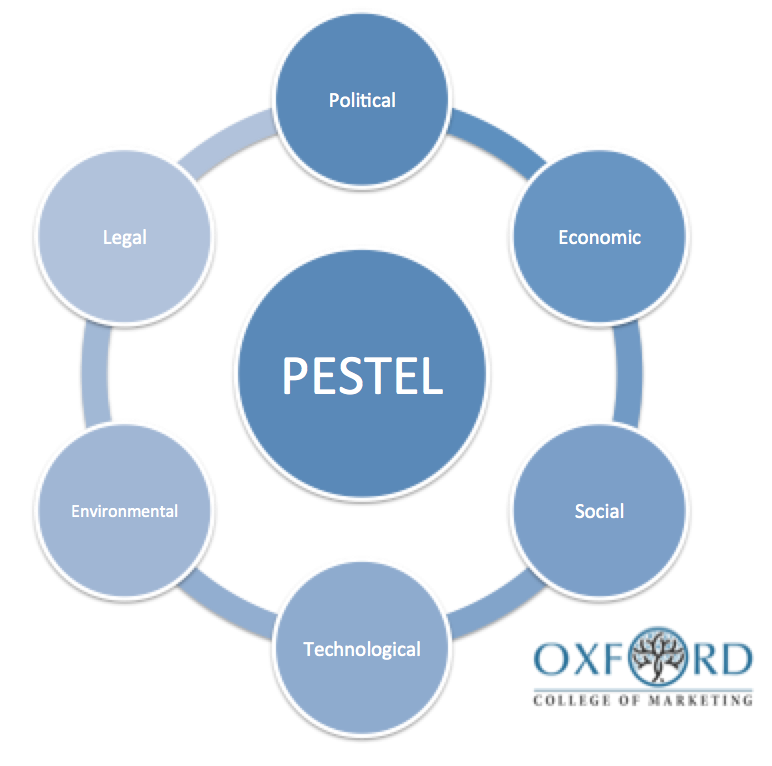
\includegraphics[width=0.5\linewidth]{figures/images/PESTEL-Analysis.png}
  \caption{Dimensiones del análisis PESTEL}
  \source{\url{https://blog.oxfordcollegeofmarketing.com/2016/06/30/pestel-analysis/}}
  \label{fig:pestel}
\end{figure}

\clearpage

\subsubsection{Análisis de las 5 fuerzas de Porter}
Este análisis fue propuesto por Michael Porter \cite{Porter1989HowStrategy}, de la Universidad de Harvard, en un artículo que data del año 1979. Proporciona un marco de reflexión estratégica en el que se identifican unas determinadas fuerzas o influencias externas dentro del entorno específico de operación que pueden afectar al desarrollo de la actividad empresarial. Estas fuerzas se representan en la Figura \ref{fig:fuerzas_porter} y son las que pueden ejercer tanto los proveedores como los clientes o la rivalidad que pueda existir entre los competidores existentes, así como las amenazas de entrada que pueden ejercer los potenciales competidores y la de los productos sustitutivos. Por tanto, se trata de una herramienta especialmente estratégica que se utiliza con el fin de elaborar planes estratégicos y modelos de negocio \cite{josemanuel}. Por tanto, este análisis resulta complementario para el análisis PESTEL puesto que, realizando ambos, se consiguen focalizar los aspectos analizados a una industria específica sin perder de vista el entorno general donde va a operar la empresa, ayudando en la toma de decisiones posterior.

\begin{figure}[h]
  \centering
  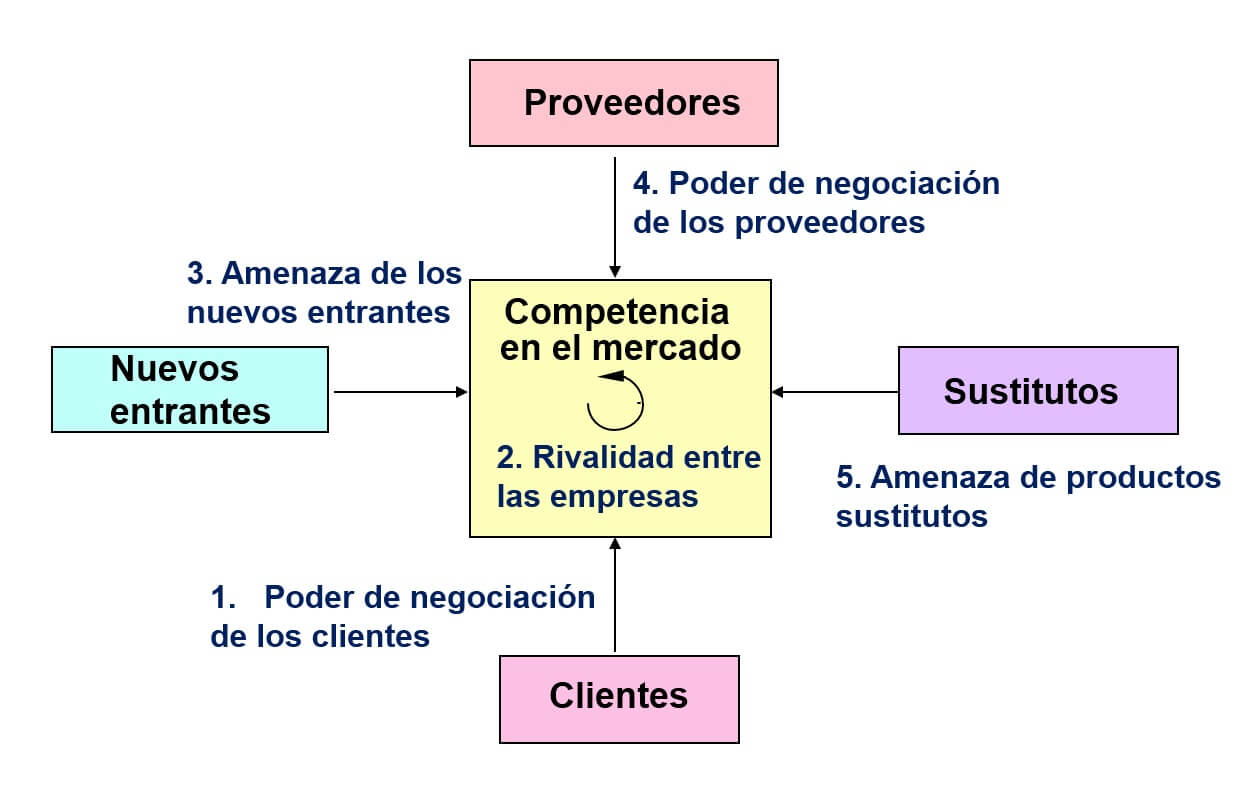
\includegraphics[width=0.75\linewidth]{figures/images/las-5-fuerzas-de-porter.jpg}
  \caption{Modelo de Porter}
  \source{\url{https://www.5fuerzasdeporter.com}}
  \label{fig:fuerzas_porter}
\end{figure}

\clearpage

\subsubsection{Lienzo del Modelo de Negocio (\textit{Business Model Canvas})}
Esta herramienta \cite{cristinaramosvega2018} fue diseñada por Alexander Osterwalder junto con Yves Pigneur y permite determinar y categorizar los diferentes elementos de una empresa con respecto a la definición de su modelo de negocio una vez se han tenido en cuenta tanto el entorno general como el específico, pues permite establecer y mantener ordenados diferentes elementos que poseen una cierta relevancia dentro de este. Esencialmente, se trata de un <<lienzo>> que permite observar de un vistazo el modelo de negocio de una empresa y se compone de nueve bloques diferenciados donde se tienen en cuenta los clientes, lo que ofrece la empresa, la infraestructura y la viabilidad económica (Figura \ref{fig:bmc}).

\begin{figure}[h]
  \centering
  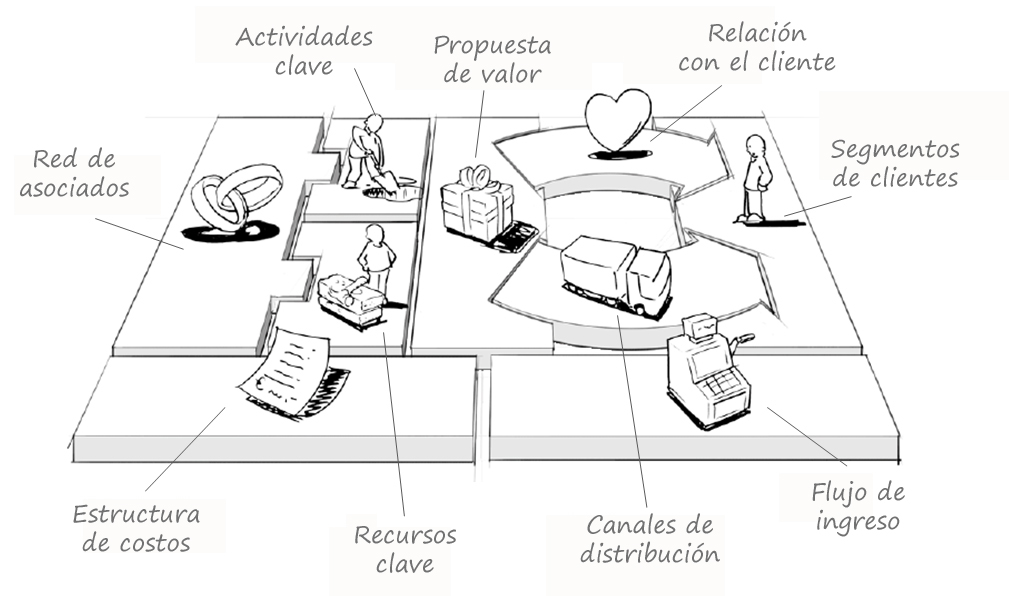
\includegraphics[width=0.8\linewidth]{figures/images/lienzo_modelos.jpg}
  \caption{Lienzo de modelos de negocio}
  \source{\url{https://www.educadictos.com/business-model-canvas/}}
  \label{fig:bmc}
\end{figure}